\chapter*{Anexo}

\section*{Prometheus}
\label{sec:appendix_prometheus}
\raggedbottom
\begin{lstlisting}[language=yaml,caption={Fichero estándar de configuración de alertas en Prometheus}, label={lst:standar.yml}]
groups:
- name: #Project_Name
  rules:

# CPU
  - alert: CPU_Warning
    expr: cpu_percentage_usage{PROJECT=""} > 90
    for: 5m
    labels:
      severity: warning
    annotations:
      summary: From {{ $labels.PROJECT }} {{ $labels.ENVIRONMENT }} the host {{ $labels.HOST }} has {{ humanize $value }}% CPU warning usage.

  - alert: CPU_Critical
    expr: cpu_percentage_usage{PROJECT=""} > 95
    for: 5m
    labels:
      severity: critical
    annotations:
      summary: From {{ $labels.PROJECT }} {{ $labels.ENVIRONMENT }} the host {{ $labels.HOST }} has {{ humanize $value }}% CPU critical usage.

# MEMORY
  - alert: Memory_Warning
    expr: memory_percentage_usage{PROJECT=""} > 90
    for: 5m
    labels:
      severity: warning
    annotations:
      summary: From {{ $labels.PROJECT }} {{ $labels.ENVIRONMENT }} the host {{ $labels.HOST }} has {{ humanize $value }}% Memory warning usage.

  - alert: Memory_Critical
    expr: memory_percentage_usage{PROJECT=""} > 95
    for: 5m
    labels:
      severity: critical
    annotations:
      summary: From {{ $labels.PROJECT }} {{ $labels.ENVIRONMENT }} the host {{ $labels.HOST }} has {{ humanize $value }}% Memory critical usage.

# FILESYSTEM/DISK
  - alert: Filesystem_Warning
    expr: filesystem_percentage_usage{PROJECT="",mountpoint!~"/mnt.*"} > 90
    for: 5m
    labels:
      severity: warning
    annotations:
      summary: From {{ $labels.PROJECT }} {{ $labels.ENVIRONMENT }} the host {{ $labels.HOST }} has {{ humanize $value }}% usage in {{ $labels.mountpoint }} [warning usage].

  - alert: Filesystem_Critical
    expr: filesystem_percentage_usage{PROJECT="",mountpoint!~""} > 95
    for: 5m
    labels:
      severity: critical
    annotations:
      summary: From {{ $labels.PROJECT }} {{ $labels.ENVIRONMENT }} the host {{ $labels.HOST }} has {{ humanize $value }}% usage in {{ $labels.mountpoint }} [critical usage].

  - alert: Filesystem_No_Exist_Critical
    expr: filesystem_exist_mountpoint{PROJECT="",mountpoint=~""} == 1
    for: 5m
    labels:
      severity: critical
    annotations:
      summary: From {{ $labels.PROJECT }} {{ $labels.ENVIRONMENT }} the host {{ $labels.HOST }} {{ $labels.mountpoint }} not found.

  - alert: Disk_Warning
    expr: disk_percentage_usage{PROJECT=""} > 90
    for: 5m
    labels:
      severity: warning
    annotations:
      summary: From {{ $labels.PROJECT }} {{ $labels.ENVIRONMENT }} the host {{ $labels.HOST }} has {{humanize $value}}% in volume {{ $labels.volume }} [warning usage].

  - alert: Disk_Critical
    expr: disk_percentage_usage{PROJECT=""} > 95
    for: 5m
    labels:
      severity: critical
    annotations:
      summary: From {{ $labels.PROJECT }} {{ $labels.ENVIRONMENT }} the host {{ $labels.HOST }} has {{humanize $value}}% in volume {{ $labels.volume }} [critical usage].

# DISK LOAD
  - alert: Disk_Load_Critical
    expr: disk_load{PROJECT=""} > 0
    for: 5m
    labels:
      severity: critical
    annotations:
      summary: From {{ $labels.PROJECT }} {{ $labels.ENVIRONMENT }} the host {{ $labels.HOST }} has excessive disk load (read/write).

# EXPORTER
  - alert: Exporter_Down_Critical
    expr: up{PROJECT=""} == 0
    for: 5m
    labels:
      severity: critical
    annotations:
      summary: From {{ $labels.PROJECT }} {{ $labels.ENVIRONMENT }} the host {{ $labels.HOST }} has the {{ $labels.EXPORTER }} is down.

# NETWORK
  - alert: Network_Warning
    expr: network_errors{PROJECT=""} > 1
    for: 5m
    labels:
      severity: warning
    annotations:
      summary: From {{ $labels.PROJECT }} {{ $labels.ENVIRONMENT }} the host {{ $labels.HOST }} has warning network problems.

  - alert: Network_Critical
    expr: network_errors{PROJECT=""} > 50
    for: 5m
    labels:
      severity: critical
    annotations:
      summary: From {{ $labels.PROJECT }} {{ $labels.ENVIRONMENT }} the host {{ $labels.HOST }} has critical network problems.

# SERVICES
  - alert: Services_Critical
    expr: service_status{PROJECT=""} == 0
    for: 5m
    labels:
      severity: critical
    annotations:
      summary: Form {{ $labels.PROJECT }} {{ $labels.ENVIRONMENT }} the host {{ $labels.HOST }} has the service {{ $labels.name }} down.
\end{lstlisting}

\section*{Diagrama UML de la aplicación}
\label{sec:appendix_uml}
%\input{include/desarrollo/uml.tex}
\begin{center}
    \begin{figure}[h]
        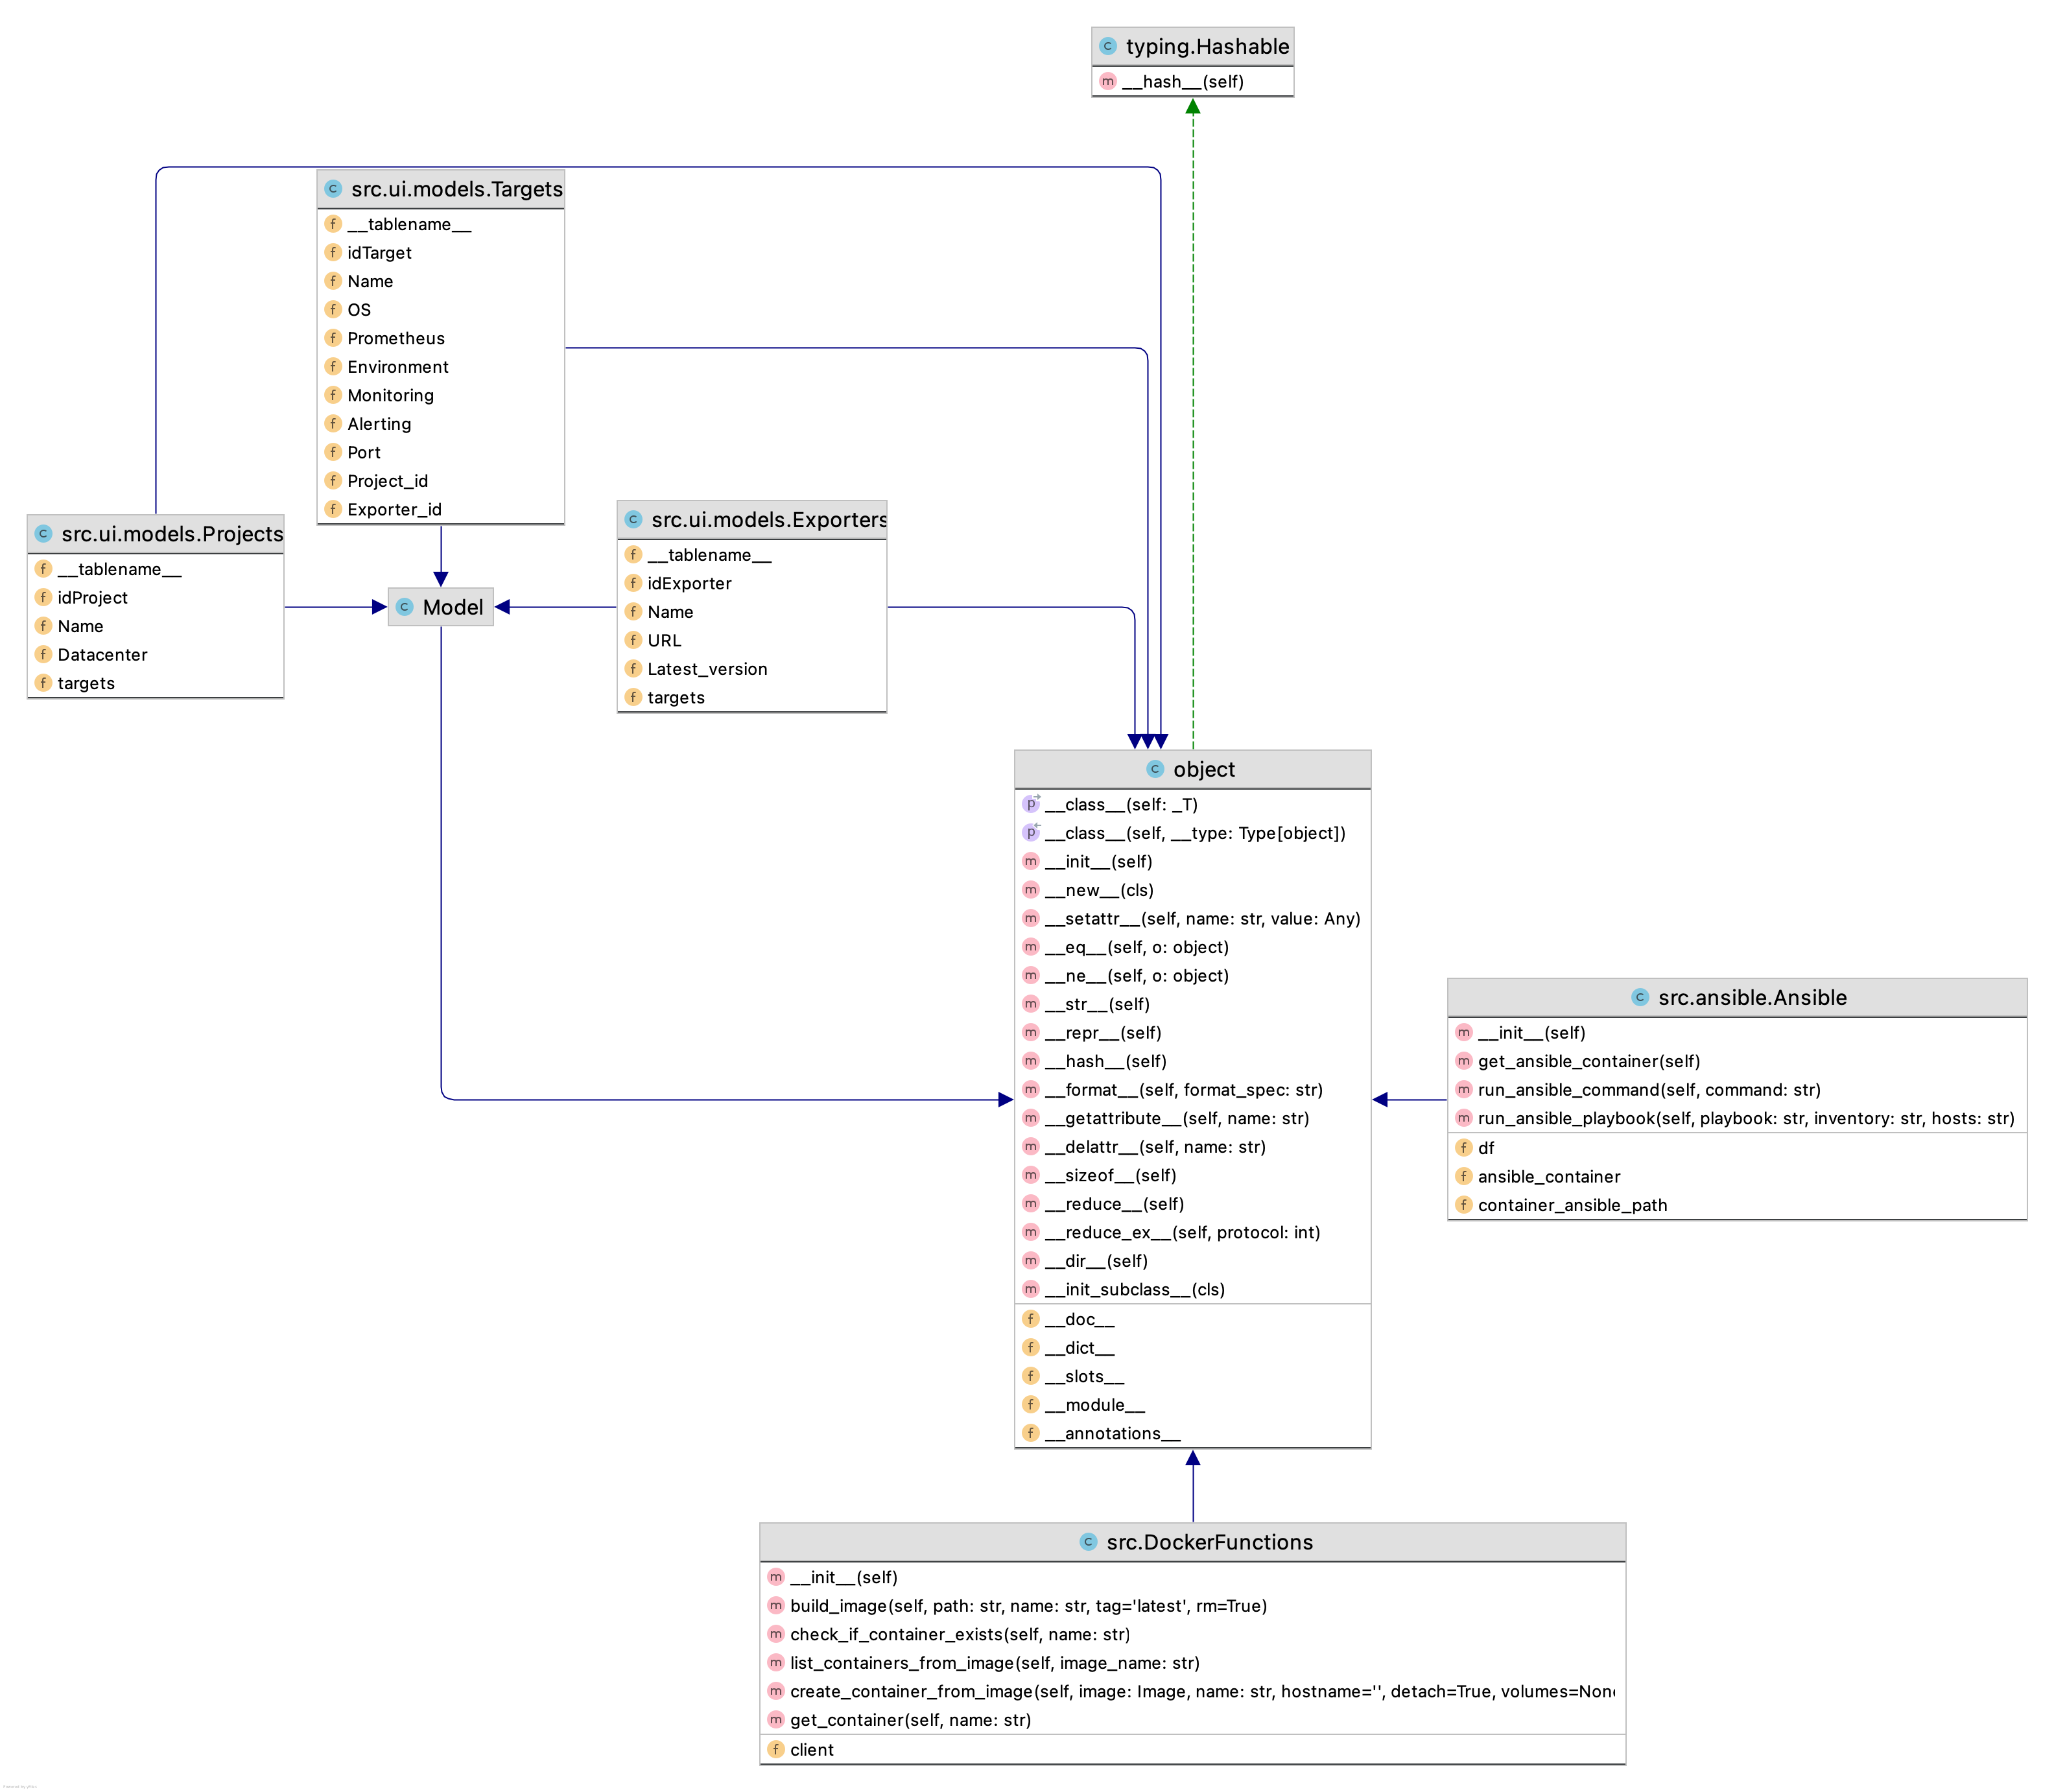
\includegraphics[width=0.9\textwidth]{include/desarrollo/src.png}
        \caption{Diagrama UML del backend}
        \label{fig:uml}
    \end{figure}
\end{center}

\section*{Ansible}
\label{sec:appendix_ansible}
\begin{lstlisting}[language=yaml,caption={Playbook creado para instalar \textit{node\_exporter}},label=lst:playbook]
- name: Install and start Node Exporter
  hosts: node_exporter
  tasks:
    - name: Create node_exporter dir
      become: yes
      file:
        path: '/opt/exporters/node_exporter'
        state: directory
        owner: root
        group: root
    - name: Install node exporter
      become: yes
      import_role:
        name: cloudalchemy.node_exporter
      vars:
        node_exporter_version: latest
        node_exporter_web_listen_address: "0.0.0.0:9100"
        node_exporter_web_telemetry_path: "/metrics"
        node_exporter_textfile_dir: "/opt/exporters/node_exporter/textfile_collector"
        node_exporter_enabled_collectors:
          - systemd
          - textfile:
              directory: "{{ node_exporter_textfile_dir }}"
        #  - filesystem:
        #      ignored-mount-points: "^/(sys|proc|dev)($|/)"
        #      ignored-fs-types: "^(sys|proc|auto)fs$"
        node_exporter_disabled_collectors: [ ]
        # Internal variables.
        _node_exporter_binary_install_dir: "/opt/exporters/node_exporter"
        _node_exporter_system_group: "prometheus"
        _node_exporter_system_user: "{{ _node_exporter_system_group }}"
\end{lstlisting}

\section*{Interfaz Gráfica}
\label{sec:appendix_gui}
\begin{figure}[H]
    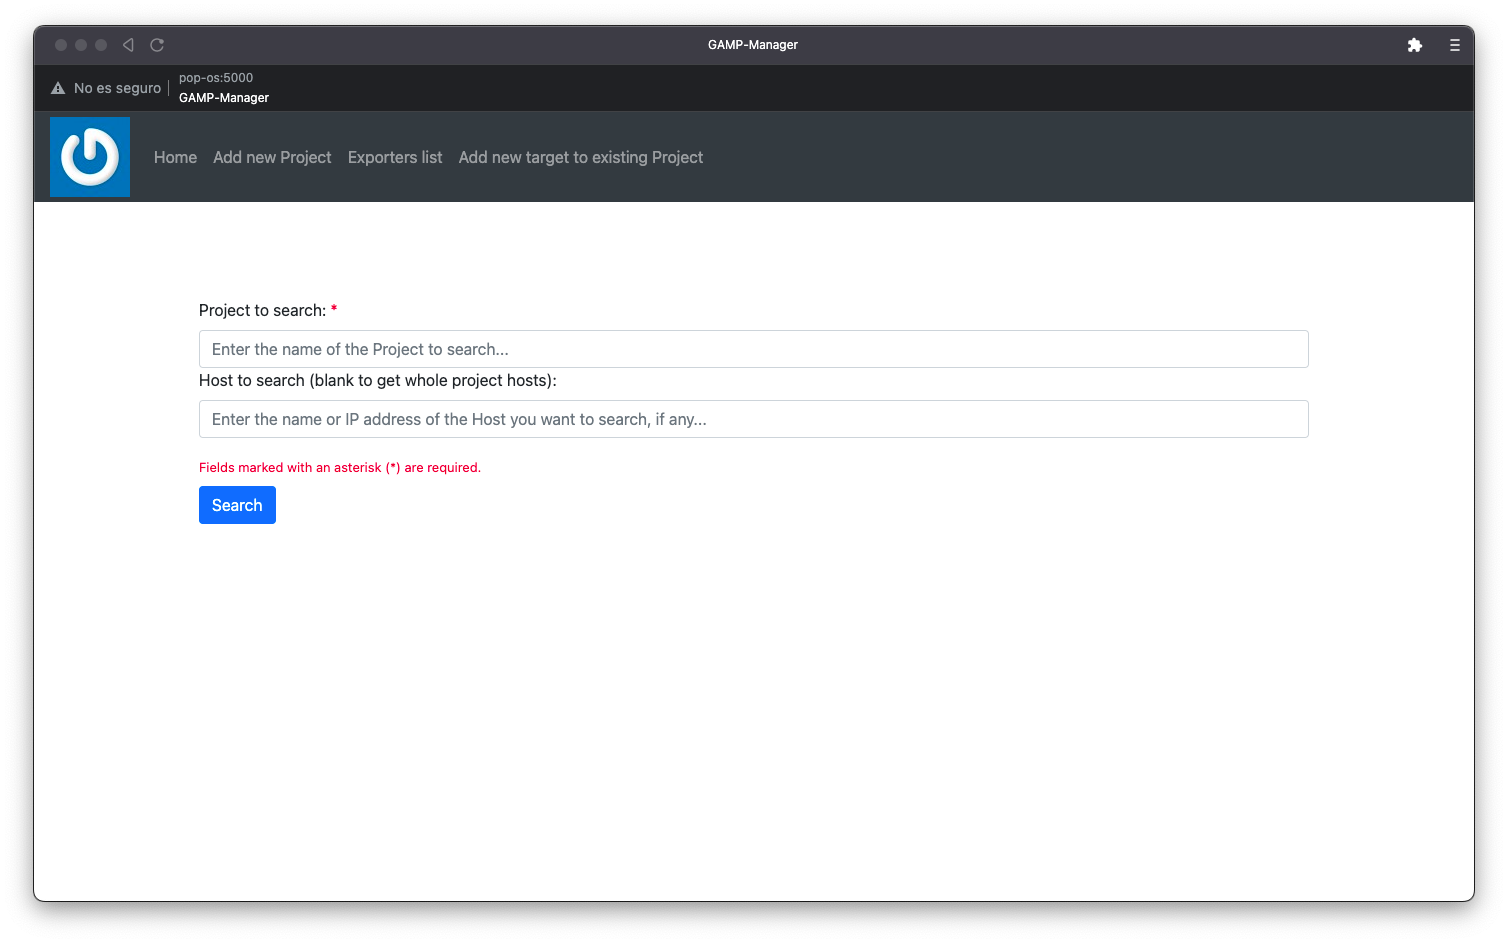
\includegraphics[width=\textwidth]{include/desarrollo/app_images/home.png}
    \caption{Página principal de selección de proyectos}
    \label{fig:gui_home}
\end{figure}

\begin{figure}[H]
    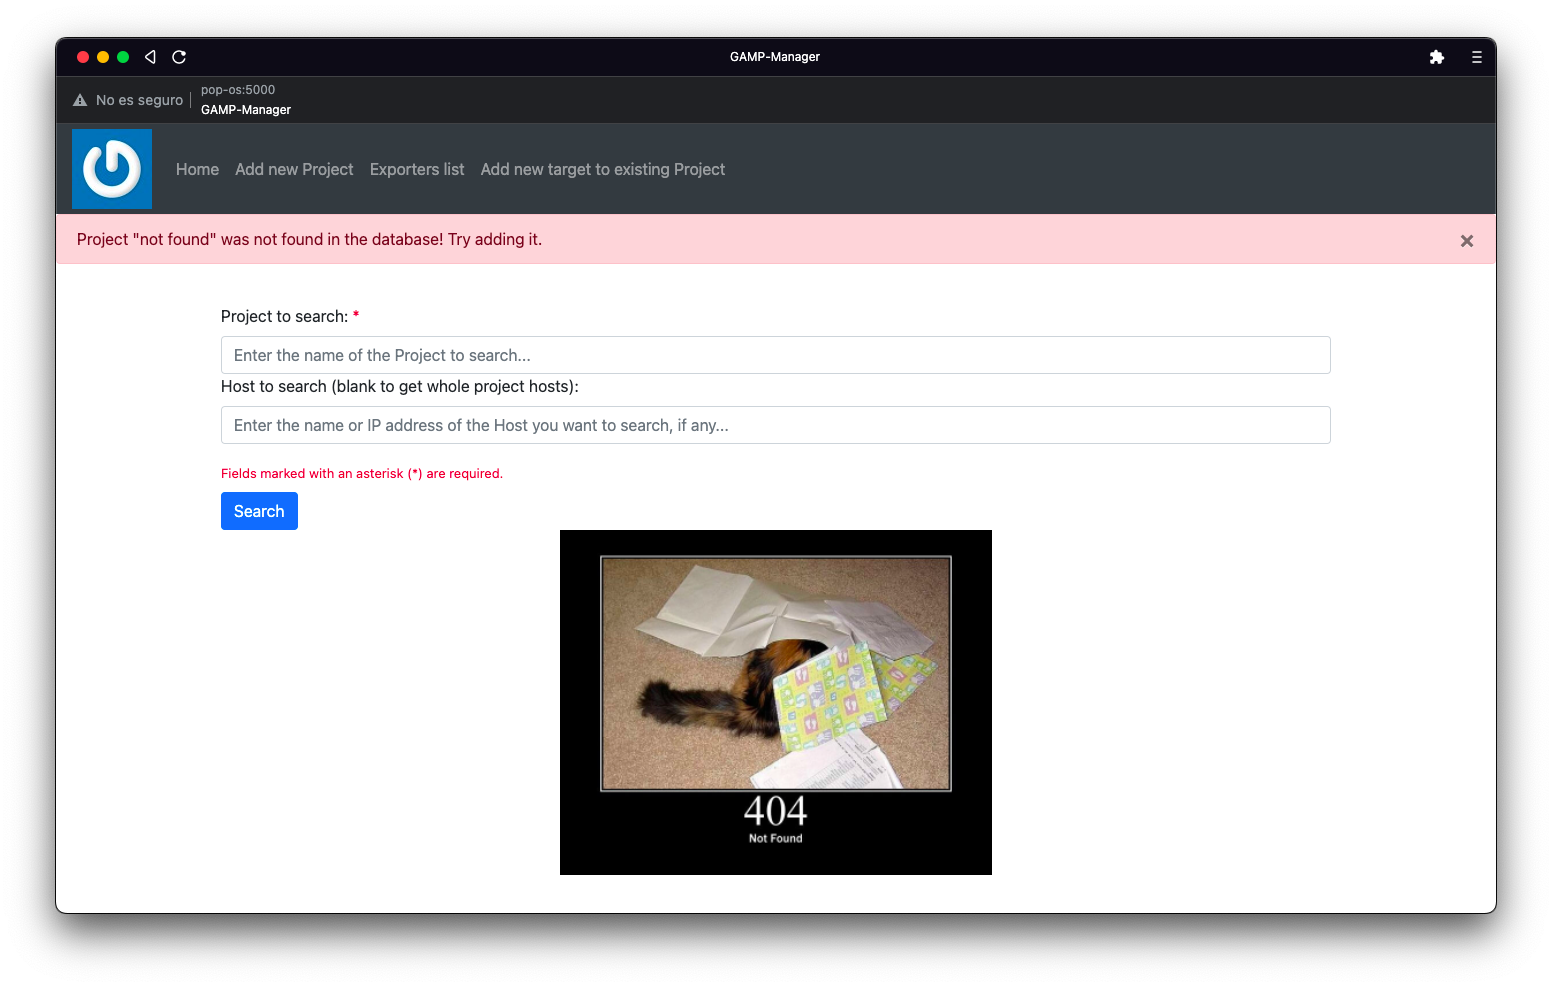
\includegraphics[width=\textwidth]{include/desarrollo/app_images/project_not_found.png}
    \caption{Proyecto no encontrado en la base de datos}
    \label{fig:gui_project_not_found}
\end{figure}

\begin{figure}[H]
    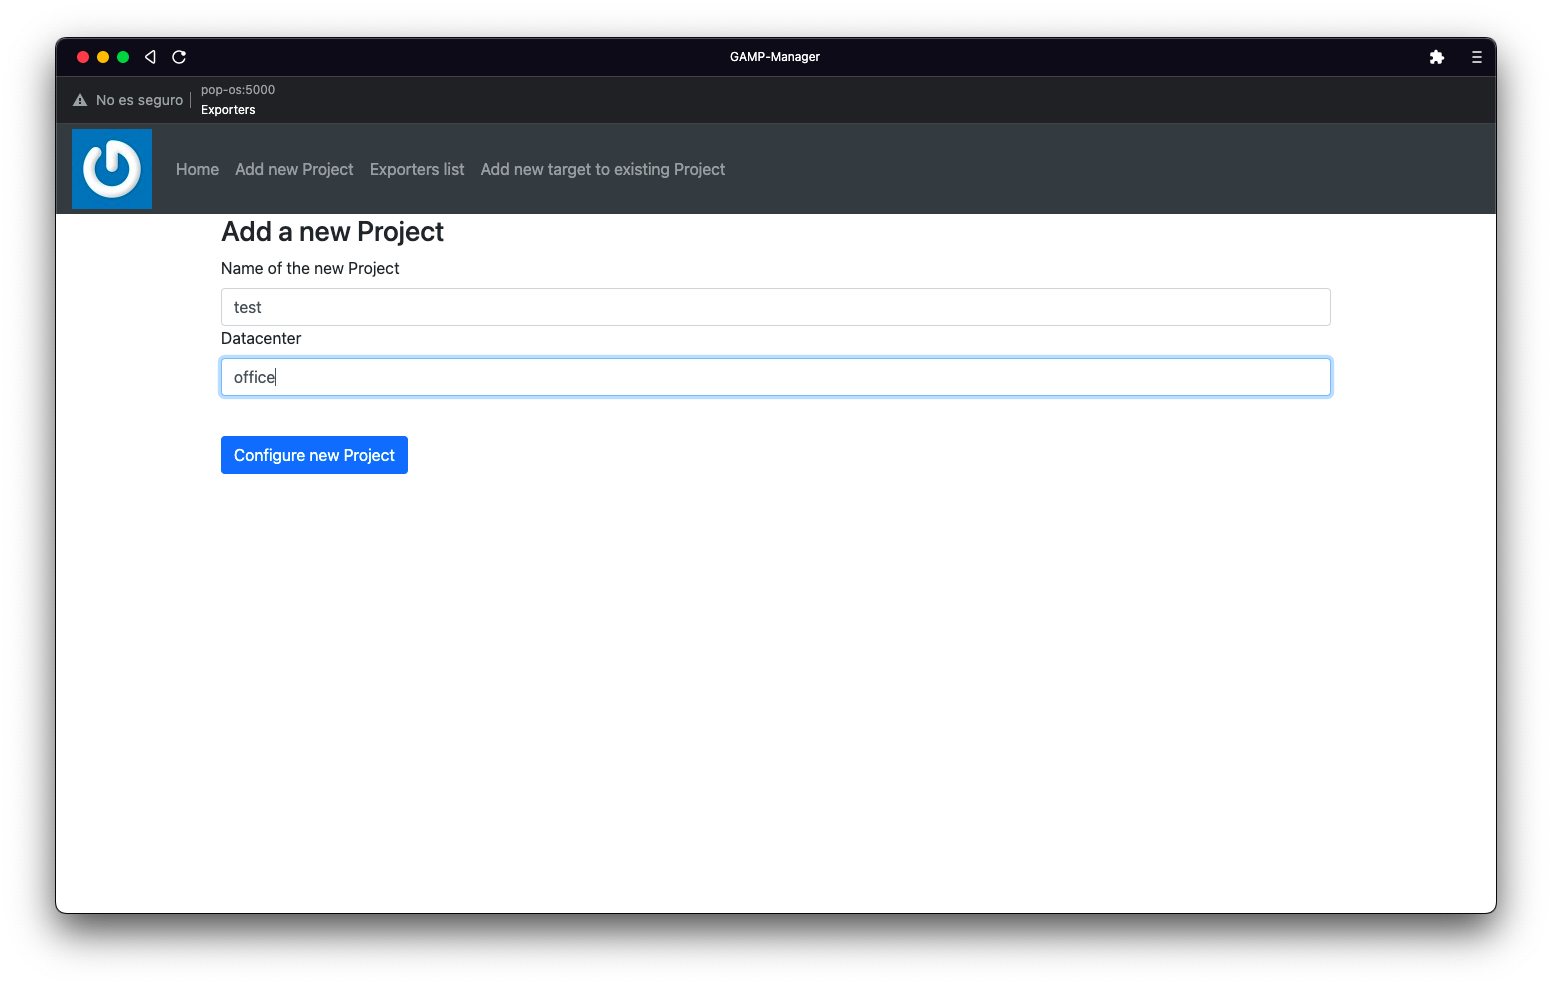
\includegraphics[width=\textwidth]{include/desarrollo/app_images/create_project.png}
    \caption{Creación de un proyecto nuevo}
    \label{fig:gui_create_project}
\end{figure}

\begin{figure}[H]
    \setbox1=\hbox{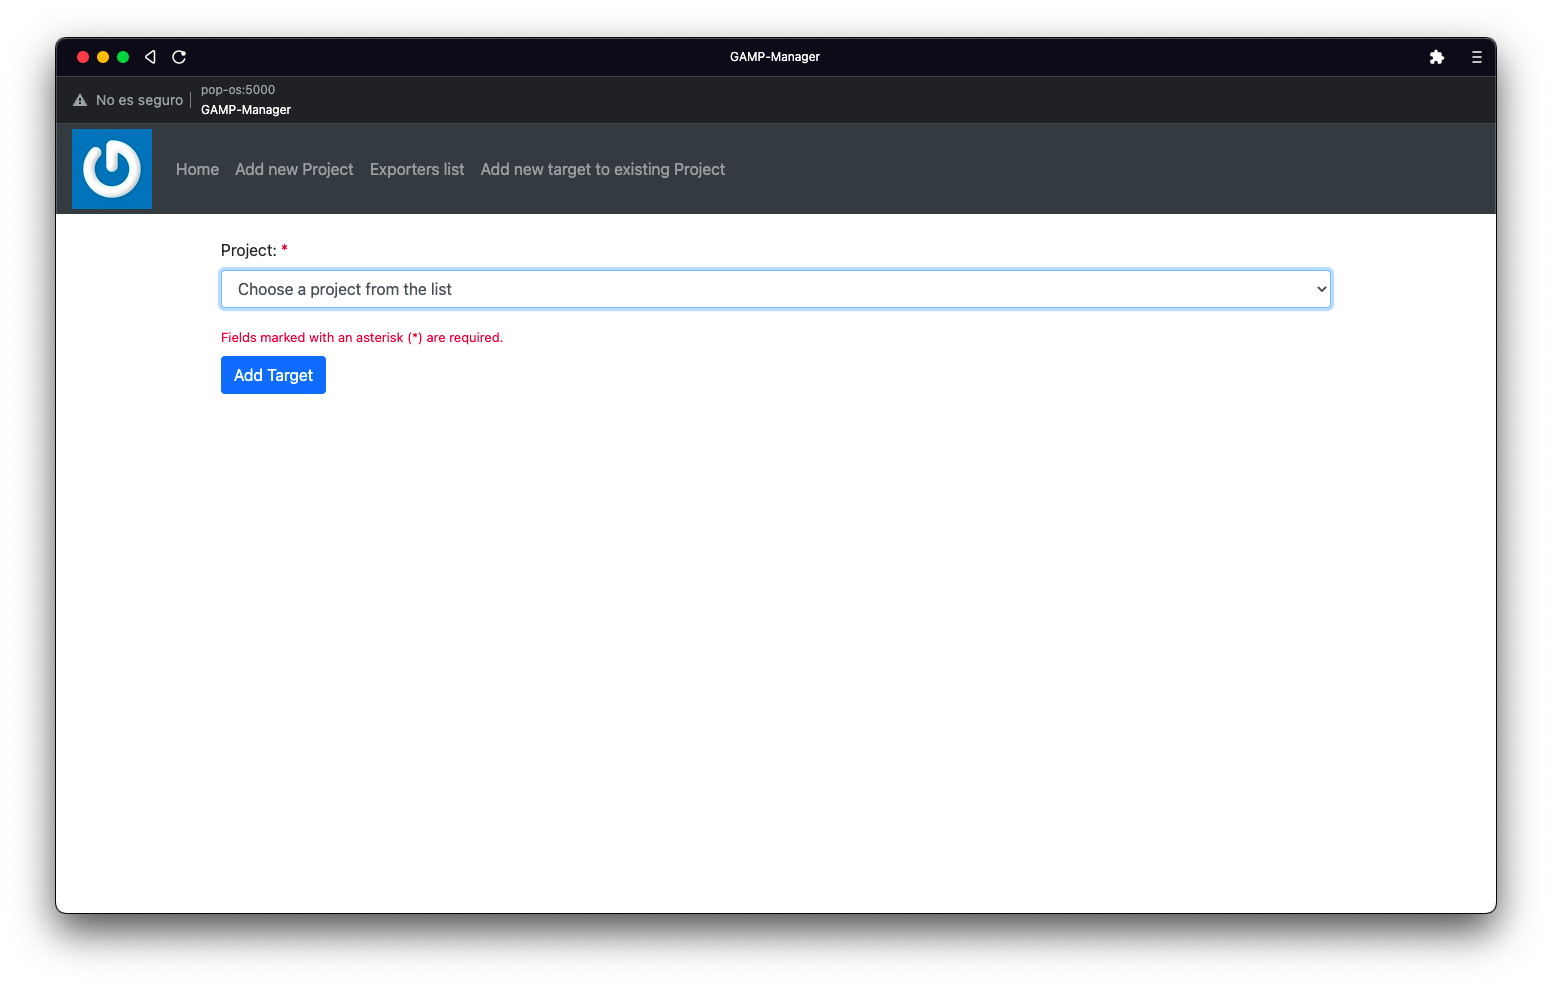
\includegraphics[width=\textwidth]{include/desarrollo/app_images/add_target_choose_project.png}}
    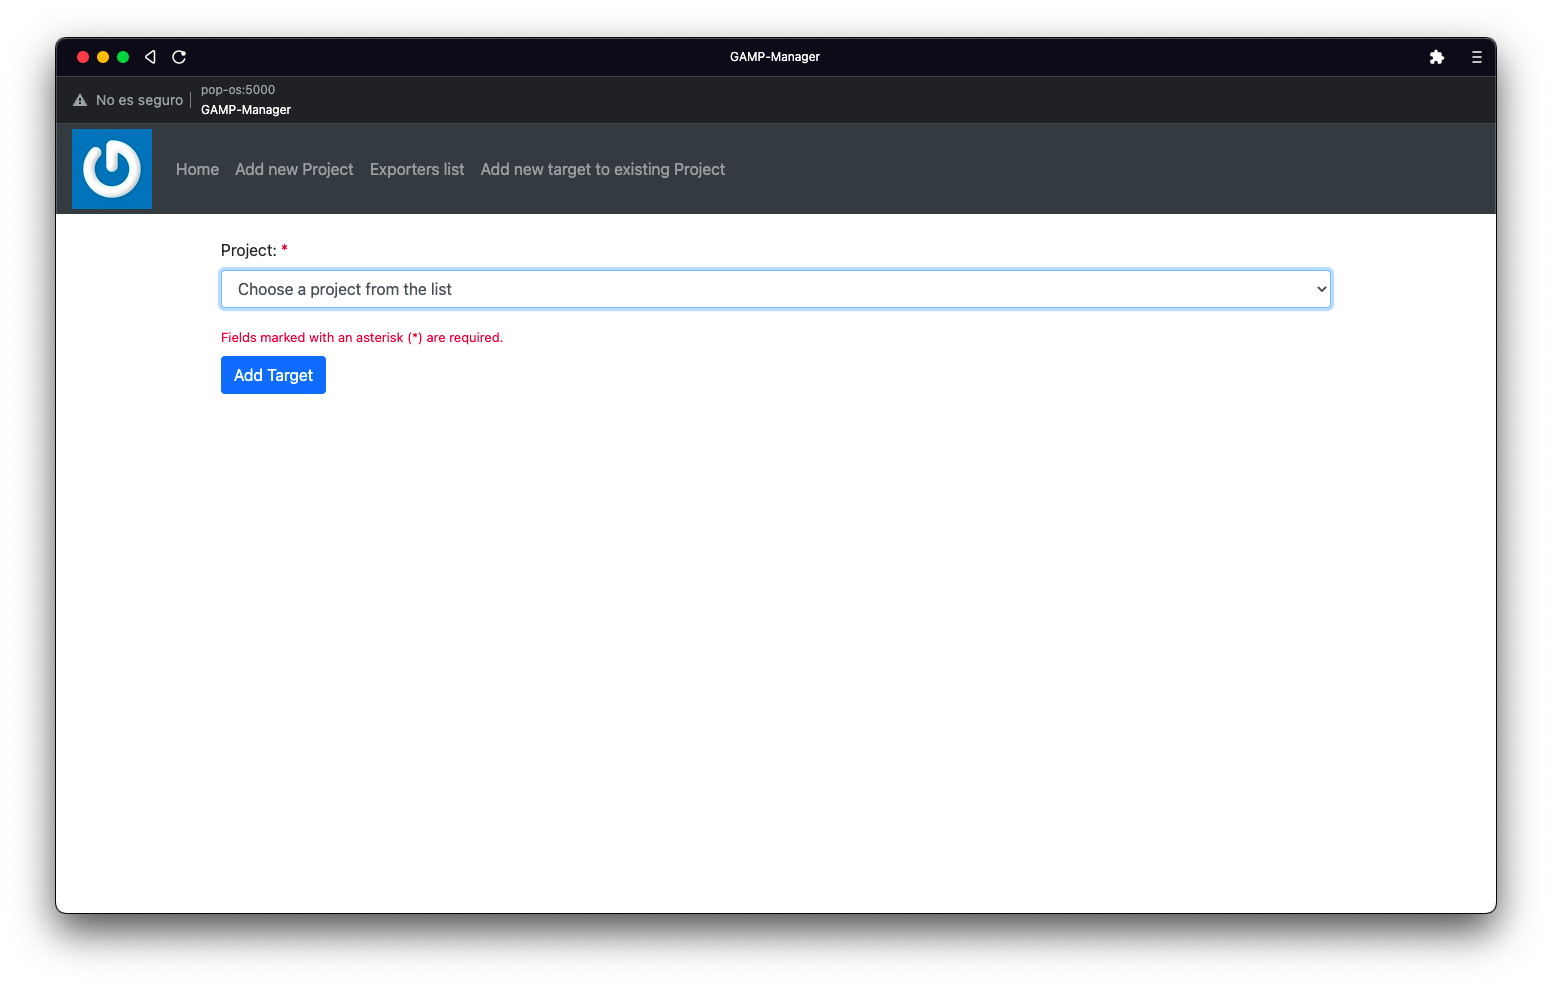
\includegraphics[width=\textwidth]{include/desarrollo/app_images/add_target_choose_project.png}\llap{\makebox[\wd1][c]{\raisebox{5.85cm}{\shifttext{-2.5cm}{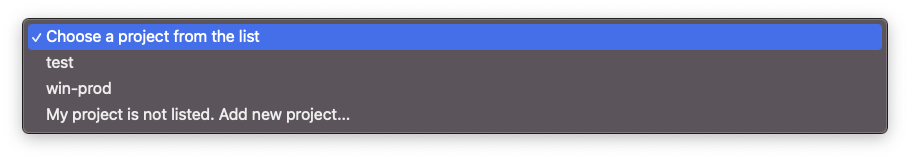
\includegraphics[width=0.6\textwidth]{include/desarrollo/app_images/project_list.png}}}}}
    \caption{Elección de proyecto para añadir	\textit{targets}}
    \label{fig:gui_add_target_choose_project}
\end{figure}

\begin{figure}[H]
    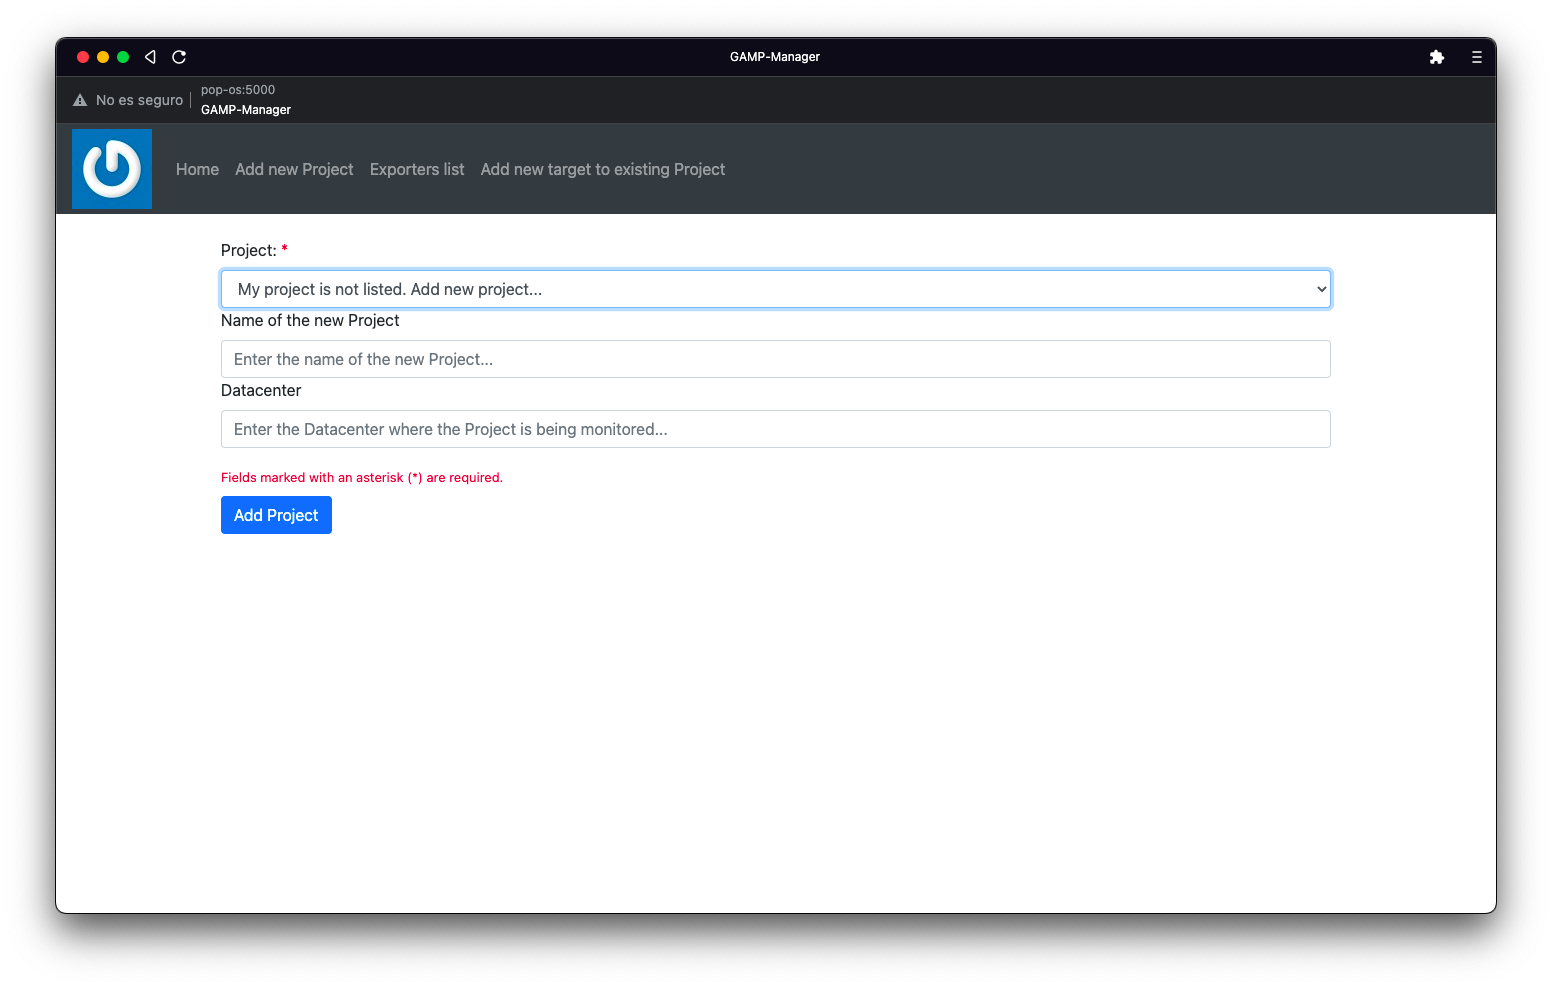
\includegraphics[width=\textwidth]{include/desarrollo/app_images/add_target_project_not_listed.png}
    \caption{Creación de un nuevo proyecto al intentar añadir	\textit{targets}}
    \label{fig:gui_add_target_project_not_listed}
\end{figure}

\begin{figure}[H]
    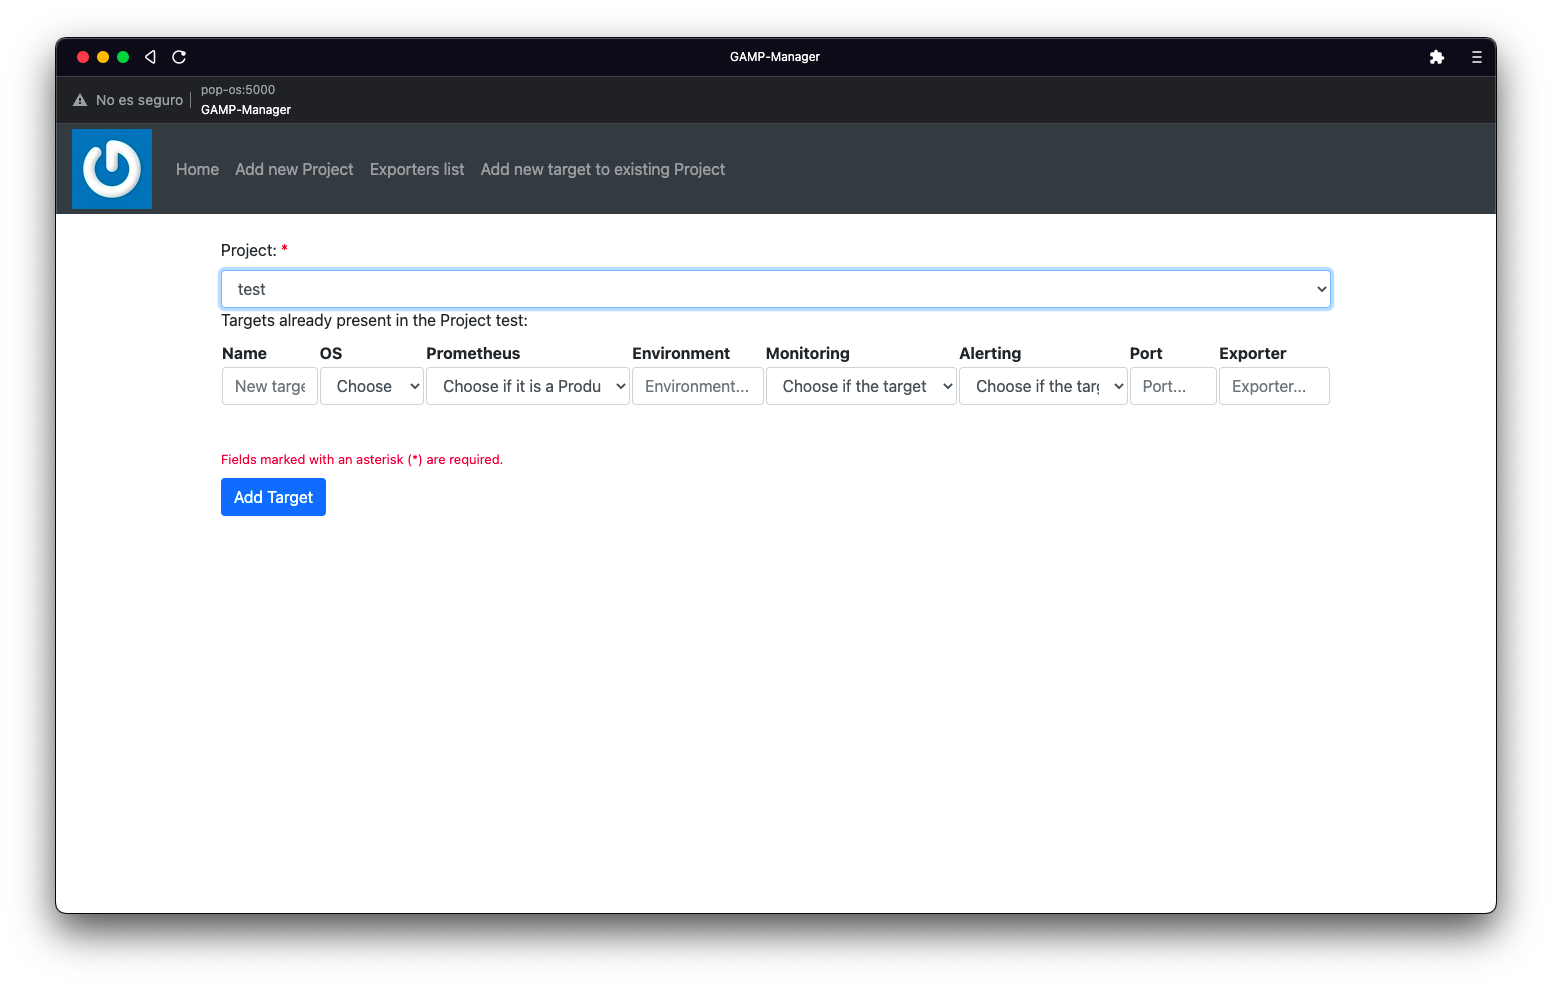
\includegraphics[width=\textwidth]{include/desarrollo/app_images/add_target_test.png}
    \caption{Creación de un target en un proyecto existente}
    \label{fig:gui_add_target_test}
\end{figure}
